% ======================================================================
% eLife submission: Genome as Projection
%
% To compile locally, download elife.cls and vancouver-elife.bst from:
%   https://www.overleaf.com/latex/templates/elife-latex-template/csqxykvsnyxm
%
% Or compile with the standard article class by uncommenting the
% fallback line below and commenting out the elife documentclass.
% ======================================================================

% --- eLife class (preferred) ---
% \documentclass[9pt,lineno]{elife}

% --- Fallback for local compilation ---
\documentclass[11pt]{article}
\usepackage[margin=1in]{geometry}
\usepackage{lineno}
\linenumbers

\usepackage{amsmath,amssymb}
\usepackage{booktabs}
\usepackage{array}
\usepackage{pdflscape}
\usepackage{graphicx}
\usepackage{hyperref}
\hypersetup{hidelinks}

\setlength{\parskip}{4pt plus 1pt minus 1pt}
\setlength{\parindent}{0pt}

% ======================================================================
% METADATA
% ======================================================================

\title{Genome as Projection: Coupling Channels Predict Cancer Survival
and Suggest Drug Response Principles}

\author{Patrick D.\ McCarthy\textsuperscript{1,*}}

% When using elife.cls, replace with:
% \author[1]{Patrick D.\ McCarthy}
% \affil[1]{Independent Researcher}
% \corr{patrick@example.com}{PM}

\date{}

\begin{document}
\maketitle

% ======================================================================
% IMPACT STATEMENT (required by eLife, 15--30 words)
% ======================================================================

\noindent\textbf{Impact statement:}
Counting disrupted organizational channels, not mutated genes,
predicts cancer survival across 73{,}593 patients and identifies
untested drug targets in 4{,}000 additional patients.

% ======================================================================
% ABSTRACT (150--200 words, third person, no subheadings)
% ======================================================================

\begin{abstract}
The genome is a linear projection of a functional graph. Genes that
appear distinct in sequence can be copies of the same functional
node, forced into separate genomic addresses by serialization
(projection families). The distributed connectivity between them,
too diffuse to encode in any single gene, constitutes coupling
channels.

Channel count predicts overall survival across 73{,}593 patients;
mutation count does not. Genes in the same projection family carry
the same drug vulnerability: expanded PARP, PI3K/AKT, and FGFR
eligibility, combination timing principles, and explanations for
published trial failures follow directly. Channel severance by any
mechanism produces predictable cancer risk: transplant
immunosuppression, neurodegeneration, information-environment
exposure.

Synthetic lethality mutual exclusivity varies fivefold across cancer
types, mapping directly to tissues where PARP inhibitors show
clinical efficacy. The co-mutation matrix alone identifies which
channels are load-bearing in which tissues.
\end{abstract}

% ======================================================================
% INTRODUCTION
% ======================================================================

\section*{Introduction}

The functional relationships between genes form a dense, cyclic
graph. The genome is a linear sequence. Serializing one into the
other forces copies: a single genomic address cannot serve all
adjacencies of a hub node. Paralogs, gene families, ``functionally
related'' genes are projection artifacts. They are copies of the
same node at different addresses.

Three claims, decreasing certainty.

\textbf{Demonstrated.} Channel count predicts survival across
73{,}593 patients ($p < 10^{-44}$). Mutation count does not. More
mutations in fewer channels means deeper commitment to one escape
route: a more constrained, treatable tumor.

\textbf{Interpretive.} A coupling channel is not a pathway. It is
the organizational function a pathway serves. Channels are the
connectivity too distributed to precipitate into any single gene.

\textbf{Predictive.} Genes in the same projection family carry the
same vulnerability. A drug that works on one works on all. Channels
severed by any mechanism produce the same cancer risk.

Channels connect cells to tissue, organ, and organism levels.
Severing them forces cell level optimization. Growth control falls
first; immune surveillance last. Formal derivations:
\cite{McCarthy2026a, McCarthy2026b, McCarthy2026c, McCarthy2026d}.
This paper can be read independently.

% ======================================================================
% RESULTS
% ======================================================================

\section*{Results}

\subsection*{Channel count predicts survival; mutation count does not}

Three publicly available datasets from cBioPortal \cite{Cerami2012}
were analyzed: the MSK-IMPACT Clinical Sequencing Cohort
($n = 7{,}091$) \cite{Zehir2017}, the MSK MetTropism Cohort
($n = 24{,}646$) \cite{Nguyen2022}, and the MSK-IMPACT 50K Cohort
($n = 41{,}856$) \cite{Bandlamudi2024}. Together: 73{,}593 patients,
28{,}750 deaths.

In multivariate Cox models, channel count is significant in every
dataset ($p < 0.005$). Mutation count either drops out (MSK-IMPACT
2017: $p = 0.67$) or becomes \emph{protective} (MetTropism:
HR $= 0.82$; 50K: HR $= 0.83$). If channel count proxied for tumor
burden, mutation count would predict worse outcomes. It predicts
better (Table~\ref{tab:empirical}, Figure~\ref{fig:km}).

\begin{figure}[ht]
\centering
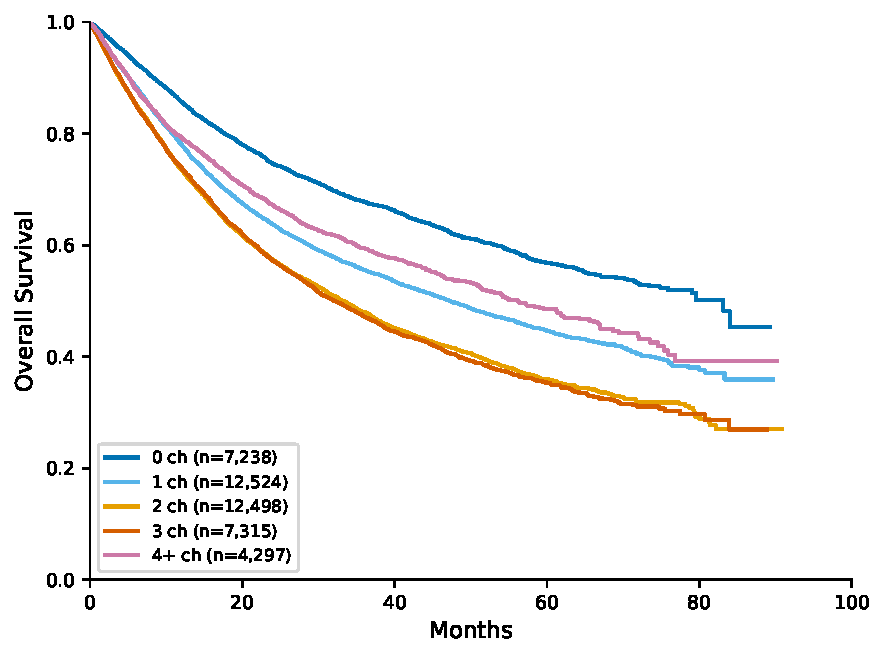
\includegraphics[width=0.85\textwidth]{figures/km_by_channel_count.pdf}
\caption{Kaplan--Meier survival curves stratified by the number of
coupling channels severed (MSK-IMPACT 50K, $n = 43{,}872$). Survival
decreases monotonically from 0 to 3 channels. The 4+ group shows
partial rebound, consistent with hypermutation phenotypes where
most mutations are passengers.}
\label{fig:km}
\end{figure}

\begin{table}[ht]
\centering
\caption{Cox proportional hazards: channel count vs.\ mutation
count across three independent cohorts totaling 73{,}593 patients.
HR = hazard ratio per unit increase. In multivariate models,
channel count remains significant while mutation count loses
predictive power or becomes protective.}
\label{tab:empirical}
\medskip
\begin{tabular*}{\textwidth}{@{\extracolsep{\fill}}llccl@{}}
\toprule
Dataset & Predictor & HR & $p$ & Note \\
\midrule
MSK-IMPACT 2017 & Channel count (univariate) & 1.10 & $<$0.005 & \\
\quad ($n=7{,}091$) & Log mutation count (univariate) & 1.12 & $<$0.005 & \\
 & Channel count (multivariate) & 1.09 & $<$0.005 & Significant \\
 & Log mutation count (multivariate) & 1.02 & 0.67 & Not significant \\
\midrule
MetTropism & Channel count (univariate) & 1.06 & $<$0.005 & \\
\quad ($n=24{,}646$) & Log mutation count (univariate) & 1.00 & 0.69 & Not significant \\
 & Channel count (multivariate) & 1.17 & $<$0.005 & Significant \\
 & Log mutation count (multivariate) & 0.82 & $<$0.005 & Protective \\
\midrule
MSK-IMPACT 50K & Channel count (univariate) & 1.04 & $<$0.005 & \\
\quad ($n=41{,}856$) & Log mutation count (univariate) & 0.98 & 0.03 & Weakly protective \\
 & Channel count (multivariate) & 1.15 & $<$0.005 & Significant \\
 & Log mutation count (multivariate) & 0.83 & $<$0.005 & Protective \\
\bottomrule
\end{tabular*}
\end{table}

Kitchen-sink Cox model with 275 covariates (TMB, MSI, cancer type,
subtype, age, sex, tumor purity, FGA, primary site, sample type,
panel version): channel count HR $= 1.09$, $p = 10^{-23}$.
MetTropism (187 covariates): HR $= 1.11$, $p = 10^{-18}$.
MSK-IMPACT 2017 (109 covariates): HR $= 1.14$, $p = 2 \times
10^{-8}$.

\subsection*{Cross-channel co-mutations are worse than same-channel}

Two mutations in different channels produce worse outcomes than
two mutations in the same channel (Table~\ref{tab:cross-channel}).
The multivariate Cox model controls for mutation count: channel
count is significant after adjustment.

\begin{table}[ht]
\centering
\small
\caption{Cross-channel vs.\ same-channel co-mutation mortality.
Cross-channel: 2+ mutations hitting different coupling channels.
Same-channel: 2+ mutations confined to one channel.}
\label{tab:cross-channel}
\begin{tabular}{@{}lrrrl@{}}
\toprule
Dataset & Cross-channel & Same-channel & $p$ (log-rank) \\
\midrule
MSK-IMPACT 2017 ($n=7{,}091$) & 33.1\% & 27.7\% &
  $1.4 \times 10^{-5}$ \\
MetTropism ($n=24{,}646$) & 42.9\% & 39.0\% &
  $6.3 \times 10^{-13}$ \\
MSK-IMPACT 50K ($n=41{,}856$) & 42.6\% & 39.7\% &
  $5.7 \times 10^{-13}$ \\
\bottomrule
\end{tabular}
\end{table}

Stratifying by fixed channel count, patients with more mutations
survive longer. At 2 channels: mortality drops from 46.2\% to
41.2\% ($p = 3.1 \times 10^{-8}$). At 3 channels: 46.9\% to
38.6\% ($p = 7.2 \times 10^{-14}$). An alternative explanation is
immunogenicity. If neoantigen load explained the protective effect,
it should also protect cross-channel patients. It does not
(Table~\ref{tab:cross-channel}). The protection is specific to
same-channel depth, not total mutation burden.

\subsection*{Synthetic lethality is tissue-conditional}

Cells that lose both copies of a functional node die. SL gene pairs
should therefore be mutually exclusive in tumors, but only where the
channel is load-bearing.

Figure~\ref{fig:sl-by-ct}: 121 SL pairs, 41 cancer types
($n = 44{,}283$). Fivefold variation. Ovarian (obs/exp $= 0.74$),
NSCLC (0.76), squamous lung (0.87): strong exclusivity. These are
where PARP inhibitors work. Colorectal (2.60), endometrial (2.97):
strong co-occurrence. Both MSI-high: mismatch repair already gone,
DDR array already failed, exclusivity constraint relaxed. The
co-mutation matrix alone maps which channels are load-bearing in
which tissues.

\begin{figure}[ht]
\centering
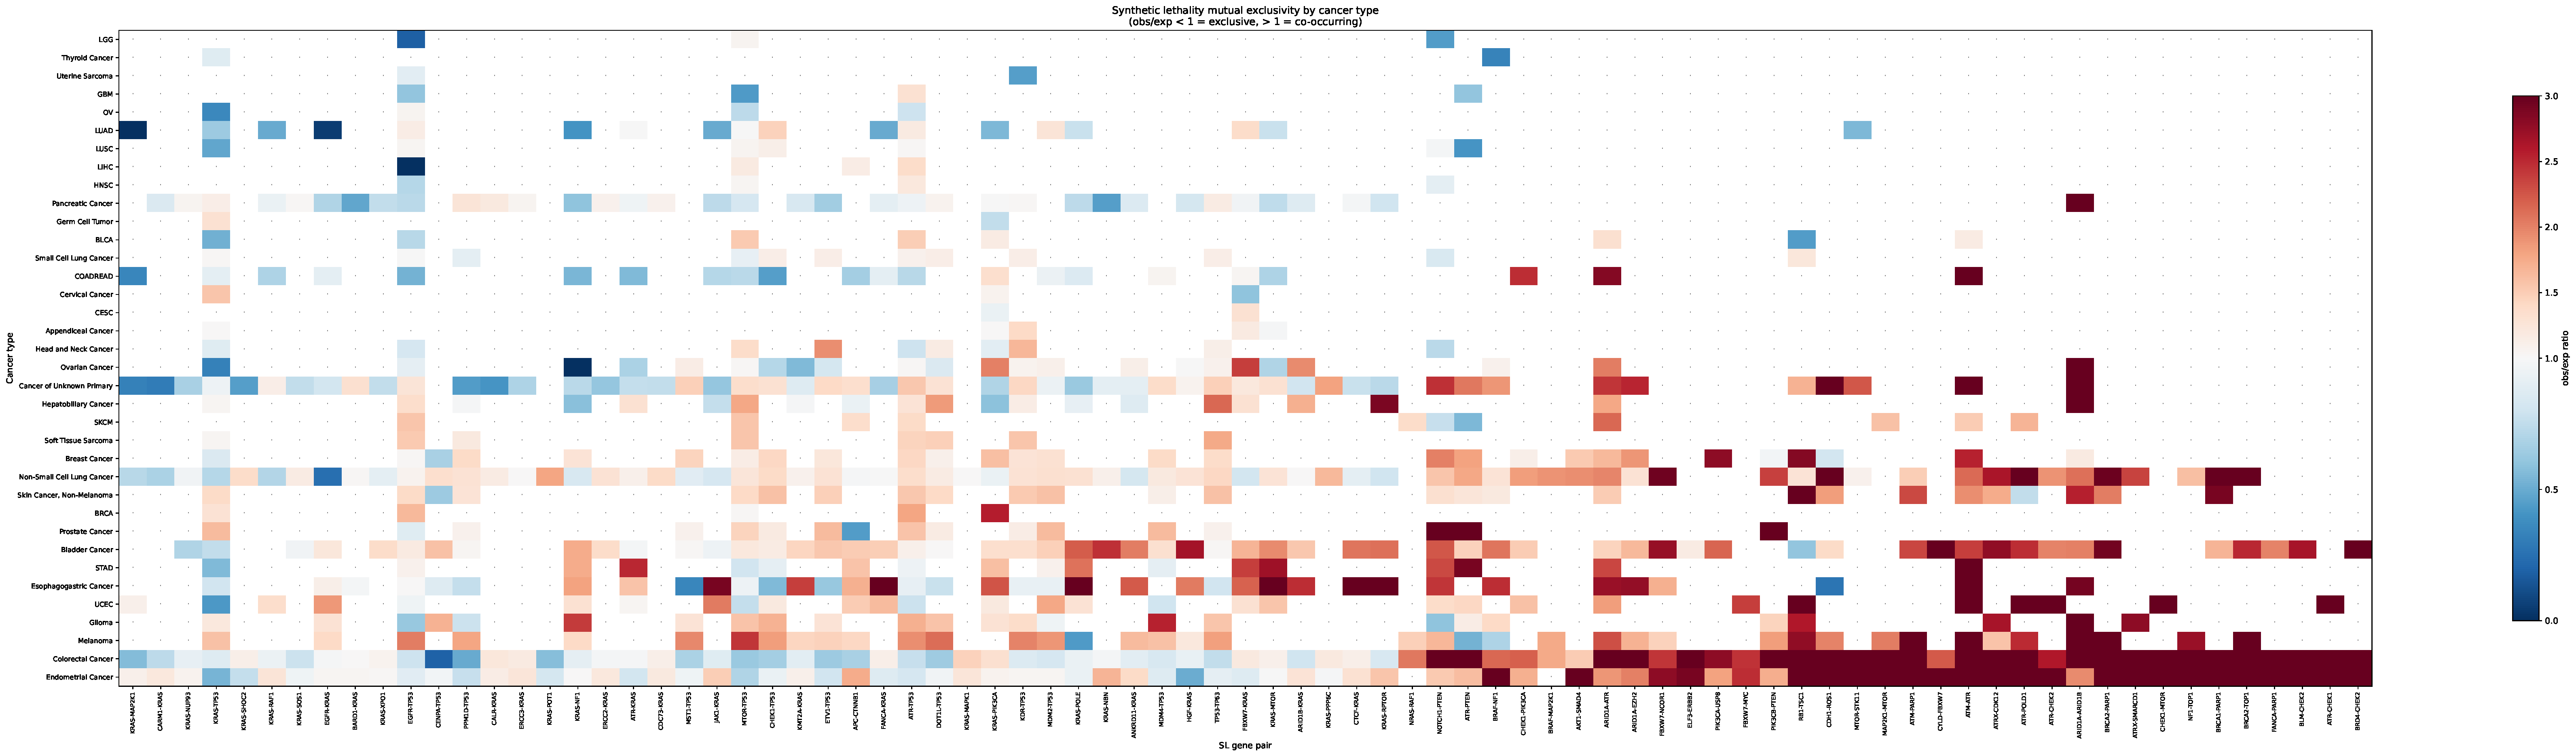
\includegraphics[width=0.95\textwidth]{figures/sl_exclusivity_by_ct.pdf}
\caption{Synthetic lethality mutual exclusivity by cancer type.
Each cell shows the observed/expected co-mutation ratio for an SL
gene pair in a given cancer type. Blue (obs/exp $< 1$): mutually
exclusive, the channel is load-bearing. Red (obs/exp $> 1$):
co-occurring, the channel is bypassed or the tumor is hypermutated.
Cancer types are sorted by mean exclusivity. The pattern predicts
where PARP inhibitors should be effective (blue rows) and where they
should not (red rows).}
\label{fig:sl-by-ct}
\end{figure}

\subsection*{Channels are tissue-specific}

Cancer type as covariate (38 types) attenuates channel count by
1.1\% (HR $= 1.17$, $p = 8 \times 10^{-73}$). Within-type: NSCLC
(HR $= 1.16$), breast (1.29), prostate (1.47), pancreatic (1.32),
all $p < 10^{-10}$. Not a proxy for cancer type.
Figure~\ref{fig:channel-by-ct}: breast is PI3K/Growth and
Endocrine. Glioma is Cell Cycle and DDR. Colorectal is Tissue
Architecture and PI3K/Growth.

\begin{figure}[ht]
\centering
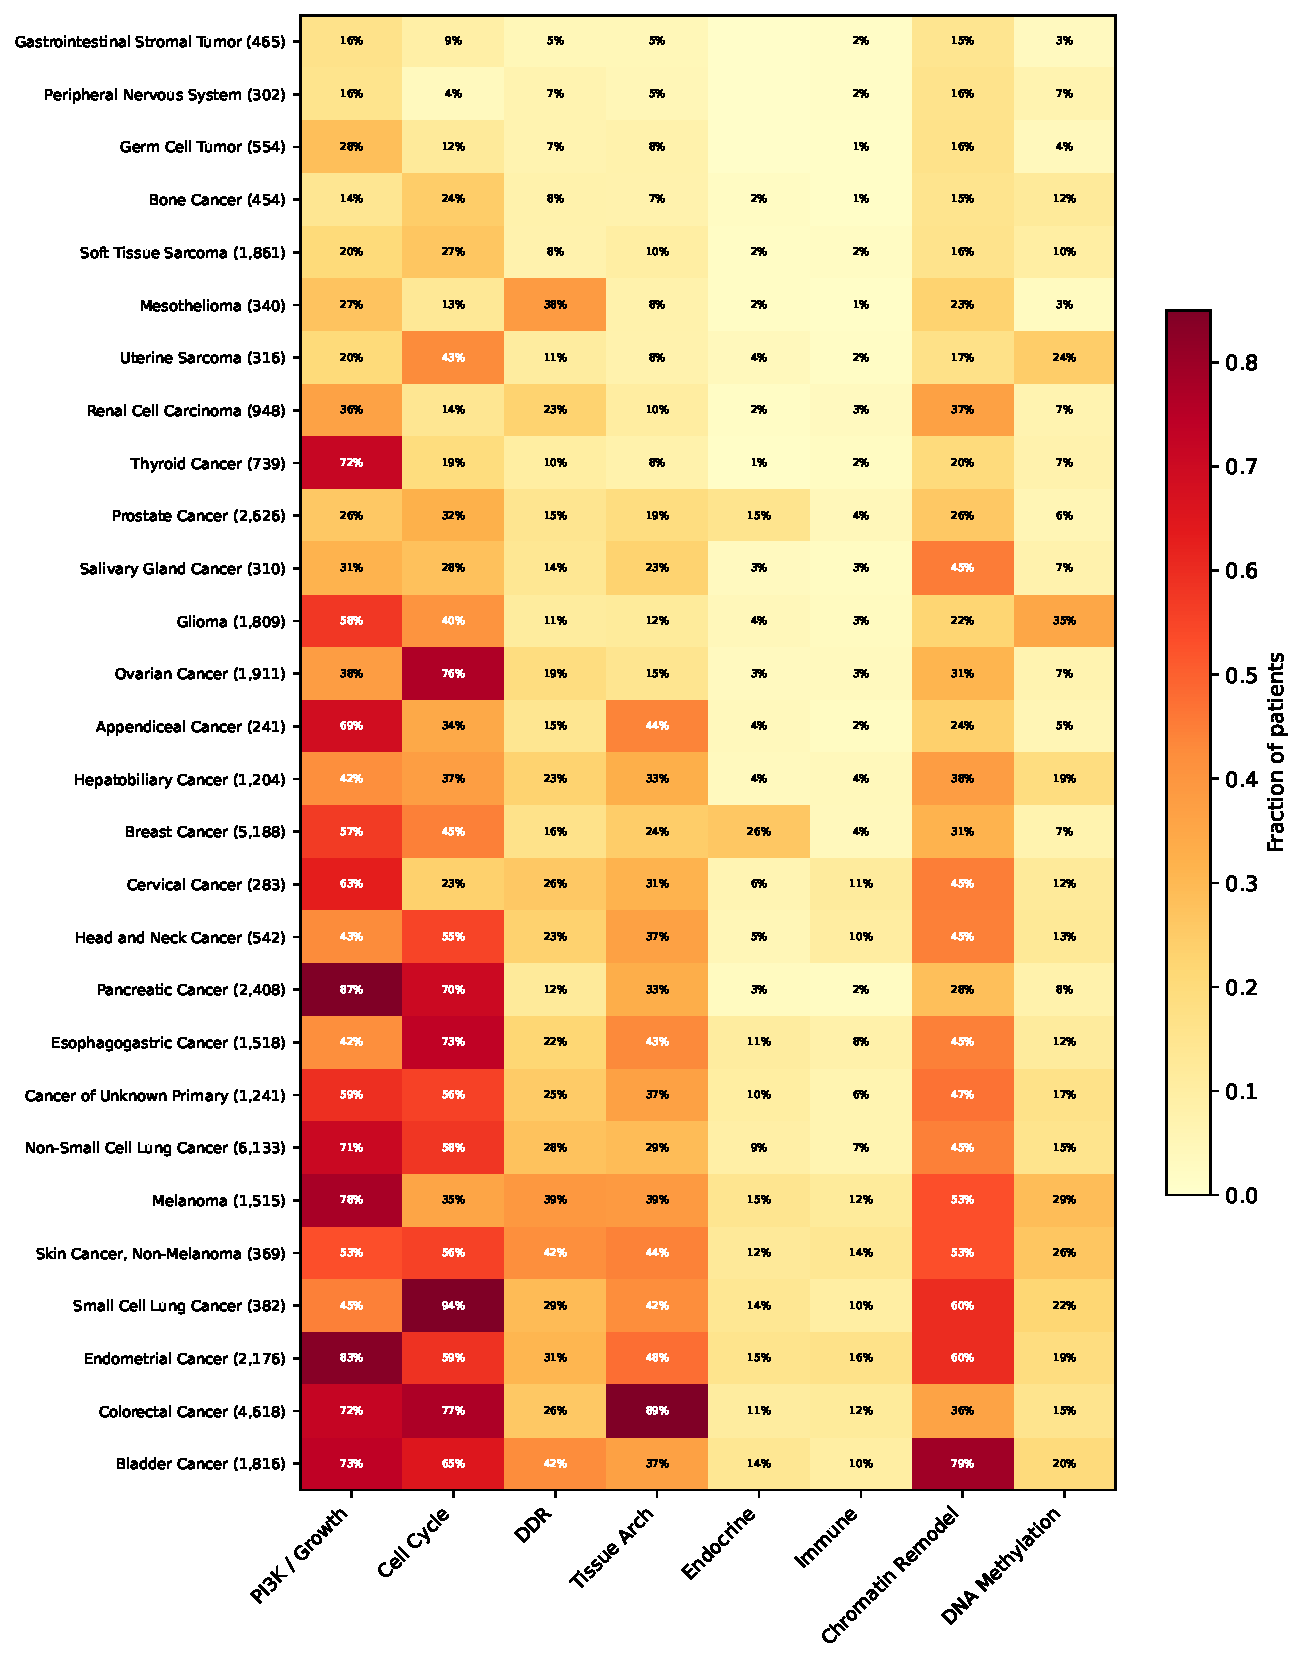
\includegraphics[width=0.95\textwidth,height=0.85\textheight,keepaspectratio]{figures/channel_frequency_by_ct.pdf}
\caption{Channel severance frequency by cancer type. Each cell
shows the fraction of patients with at least one mutation in the
given channel. Cancer types sorted by total channel burden. Breast
is Endocrine-dominant, colorectal is Tissue Architecture-dominant,
glioma is Cell Cycle-dominant.}
\label{fig:channel-by-ct}
\end{figure}

\subsection*{Severance hierarchy: cell-intrinsic channels first}

Not random (Figures~\ref{fig:hierarchy},~\ref{fig:coseverance}).
One channel severed ($n = 12{,}558$): 80\% PI3K/Growth or Cell
Cycle. Endocrine and Immune: under 5\%.

PI3K/Growth $\to$ Cell Cycle $\to$ Tissue Architecture $\to$
DDR $\to$ Endocrine $\to$ Immune. Growth escape is the gateway;
immune evasion is last. The co-severance matrix
(Figure~\ref{fig:coseverance}) is asymmetric: cell-intrinsic
severance predicts organism-level, not the reverse.

\begin{figure}[ht]
\centering
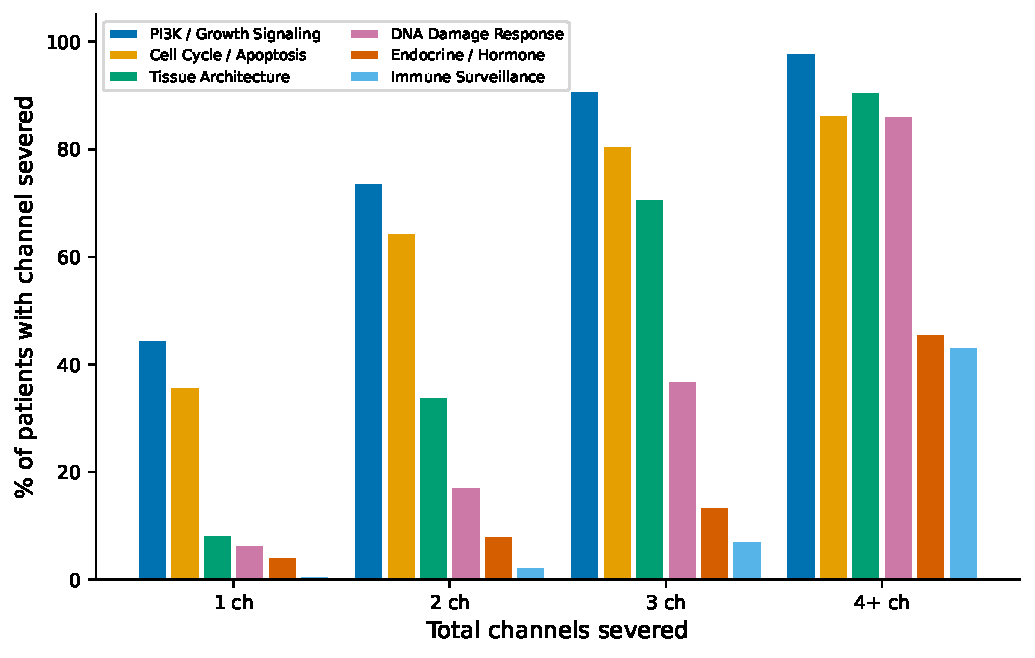
\includegraphics[width=0.9\textwidth]{figures/severance_hierarchy.pdf}
\caption{Severance hierarchy across channel-count strata
(MSK-IMPACT 50K). Each bar shows the percentage of patients at a
given stratum who have that channel severed. Cell-intrinsic channels
dominate at every stratum; organism-level channels appear only at
higher channel counts.}
\label{fig:hierarchy}
\end{figure}

\begin{figure}[ht]
\centering
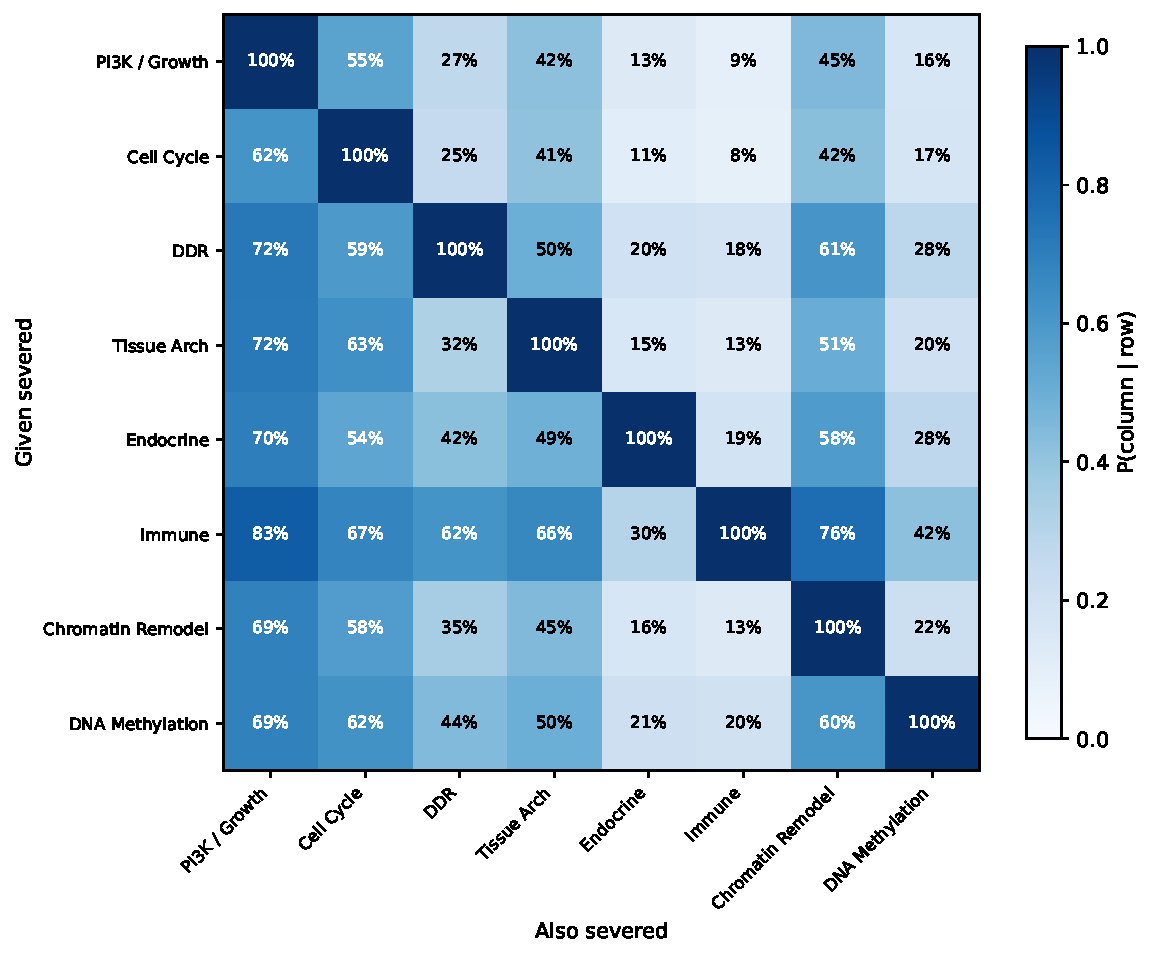
\includegraphics[width=0.7\textwidth]{figures/channel_coseverance.pdf}
\caption{Channel co-severance matrix. Each cell shows
P(column channel severed $\mid$ row channel severed). The matrix is
asymmetric: cell-intrinsic channels predict organism-level severance,
but not the reverse. Severance propagates inward toward the root of
the escalation hierarchy.}
\label{fig:coseverance}
\end{figure}

1.9\% of multi-channel patients lack a cell-intrinsic gateway.
Enriched 6.5$\times$ for prostate, 2.5$\times$ breast,
7.6$\times$ mesothelioma: cancers entering through organism level
channels. Lower mortality (34.8\% vs.\ 42.6\%). They never escaped
the most fundamental coupling layer.

\subsection*{Sensitivity and robustness}

The signal peaks at 3 channels ($p = 3 \times 10^{-124}$) and is
significant from 2 through 8 (Table~\ref{tab:sensitivity}). At 10,
over-splitting collapses channel count back into a proxy for mutation
count. Hierarchical clustering on Jaccard co-mutation distances
produces groupings that fail: at $k = 6$, HR $= 0.80$
($p = 9 \times 10^{-6}$), the wrong direction. Biological channels
at $k = 6$: HR $= 1.10$ ($p = 3 \times 10^{-9}$). ARI between
data-driven and biological groupings: 0.018. Co-mutation clusters
group genes by which tumors they appear in. Channels group genes by
which organizational system they serve.

\begin{table}[ht]
\centering
\caption{Sensitivity analysis (MSK-IMPACT 50K, $n = 41{,}856$):
multivariate Cox hazard ratios at different channel granularities.}
\label{tab:sensitivity}
\medskip
\begin{tabular*}{\textwidth}{@{\extracolsep{\fill}}rcccc@{}}
\toprule
Channels & Ch HR & Ch $p$ & Mut HR & Mut $p$ \\
\midrule
2 & 1.25 & $2 \times 10^{-52}$ & 0.94 & $4 \times 10^{-9}$ \\
3 & 1.30 & $3 \times 10^{-124}$ & 0.86 & $8 \times 10^{-41}$ \\
4 & 1.21 & $3 \times 10^{-75}$ & 0.88 & $9 \times 10^{-27}$ \\
5 & 1.17 & $8 \times 10^{-58}$ & 0.88 & $6 \times 10^{-22}$ \\
6 & 1.14 & $1 \times 10^{-44}$ & 0.90 & $2 \times 10^{-16}$ \\
7 & 1.10 & $7 \times 10^{-24}$ & 0.93 & $1 \times 10^{-7}$ \\
8 & 1.07 & $3 \times 10^{-14}$ & 0.95 & $4 \times 10^{-4}$ \\
10 & 1.01 & 0.064 & 1.02 & 0.20 \\
\bottomrule
\end{tabular*}
\end{table}

Restricting to truncating mutations strengthens the signal:
HR rises from 1.15 to 1.19 ($p = 10^{-55}$). MSK-IMPACT sequences
400--500 genes, systematically undercounting channel hits. This works
against the hypothesis, not for it.

\subsection*{Predictions from the projection framework}

\textbf{DDR family: PARP eligibility expansion.}
Current trials screen for 9 DDR genes. Ten additional genes share
the same functional role: \emph{BLM}, \emph{NBN}, \emph{ERCC4},
\emph{CHEK1}, \emph{CHEK2}, \emph{RAD51B}, \emph{RAD51},
\emph{BRIP1}, \emph{MRE11}, \emph{XRCC2}. Over 4{,}000 patients in
the MSK-IMPACT cohort. None currently eligible for PARP trials.

\textbf{PI3K and FGF family expansion.} \emph{INPP4B},
\emph{PIK3CB}, \emph{PIK3CD}: AKT inhibitor sensitivity comparable
to \emph{PTEN}-loss. \emph{FGFR4}: pan-FGFR inhibitor response.
\emph{CREBBP} and \emph{EP300} (3{,}491 combined patients):
functionally equivalent, same future targeted therapy.

\textbf{Same-channel combinations fail.} PARP + ATR, PARP + WEE1,
PARP + ATM, dual PARP1/2 versus PARP1-selective: no significant PFS
improvement over the simpler regimen. Two drugs in one channel add
dose, not a new therapeutic axis.

\textbf{Cross-channel timing matters.} Metastatic HR+ breast cancer
post-endocrine progression: adding a SERD to a PARP inhibitor buys
little. The endocrine channel is already gone. Adjuvant setting,
different story: low-dose PARP1-selective alongside endocrine therapy
in germline DDR carriers. The PARP kills cells at DDR second-hit
before they evolve ESR1 resistance. The endocrine therapy keeps the
channel open. Each drug extends the other. PARP1-selective agents
eliminate PARP2-driven hematological toxicity, enabling long-term
adjuvant dosing.

\textbf{Natural PARP1 disruption.} \emph{PARP1} loss-of-function
alongside DDR partner mutations: the genome produced the same
synthetic lethality the drug exploits. These patients should show
improved survival without PARP inhibitor treatment.

\textbf{Graph position determines phenotype.} Hub mutations carry
worse prognosis than leaf mutations in the same channel. BRCA1 (DDR
hub) drives triple-negative breast cancer. BRCA2 (DDR leaf) drives
HR+. RAD51C phenocopies BRCA2, not BRCA1. GOF and LOF in the same
gene produce opposite signatures.

\textbf{Severance is directional at two scales.} Across channels:
growth first, immune last (Figure~\ref{fig:coseverance}). Within
channels: leaves before hubs (\emph{CDK4} before \emph{TP53},
\emph{BRCA2} before \emph{BRCA1}, \emph{BRAF} before \emph{KRAS}).
Reverse direction at either scale: rare, better prognosis.

\textbf{Non-genetic severance.} Transplant immunosuppression severs
the immune channel artificially. Cancer risk elevates in
immune-dependent types, not uniformly \cite{Engels2011}.
Parkinson's: reduced cancer risk (context-switching machinery
disabled, fewer DNA damage events). ADHD: elevated cancer risk
(excessive switching, chromatin damage accumulates). Stimulants
should reduce it. Early-onset cancers in young adults: enriched for
chromatin remodeling mutations.

Companion papers: \cite{McCarthy2026f} (graph position),
\cite{McCarthy2026h} (non-genetic severance).

% ======================================================================
% DISCUSSION
% ======================================================================

\section*{Discussion}

\subsection*{Genome as projection}

Serialization forces three compromises. Cycles must be broken:
feedback loops are severed during projection and reconstructed at
runtime via transcription factors, signaling cascades, chromatin
looping. These reconstructed edges are the most fragile. Hub nodes
must be copied: a single address cannot serve all adjacencies. What
appears as genetic diversity is serialization overhead. Distributed
connectivity cannot be written at all. Channels exist only in the
three dimensional fold of the chromatin: unprecipitated knowledge,
reconstructed by physical proximity when the helix folds.

\subsection*{Chain severance}

A cell maintains finite regulatory states ($C_n$) \cite{Cowan2001}.
Multicellularity overcomes this by hierarchical coupling: cell to
tissue to organ to organism \cite{McCarthy2026b}. Channels are the
dimensions: gap junctions \cite{Aasen2016}, paracrine signaling,
endocrine and immune \cite{Hanahan2011}.

Lose a channel and the cell's context contracts. What remains:
proliferation, metabolic autonomy, motility. Hanahan and Weinberg's
hallmarks \cite{Hanahan2011} are not acquired capabilities. They are
what a cell does when it can no longer hear the tissue. The Warburg
effect is not a metabolic choice; it is what happens when oxygen
supply information is gone \cite{Warburg1956}.

\subsection*{Projection families}

The genome maintains redundant copies of critical subgraphs like a
RAID array. Lose one copy and the system degrades. Remove the parity
check (the synthetic lethal partner) and the degraded array fails.

A PARP inhibitor works regardless of which DDR copy is broken:
BRCA1, BRCA2, RAD51C. The drug targets function, not address.
Severance occurs through multiple mechanisms: genetic,
microenvironmental, epigenetic, spatial
(Table~\ref{tab:severance-mechanisms}). All produce the same
endpoint. This is why hereditary, environmental, and sporadic
cancers converge.

\subsection*{Prior work}

TOFT \cite{Sonnenschein2000} got the level right (tissue, not cell)
and the default state right (proliferative). It lacked formalism.
The escalation chain provides it. No existing cancer model addresses
projection. Current frameworks treat genes as independent entities
in shared pathways. They are copies of shared nodes. Different
question, different answer to ``target a gene.''

\subsection*{Limitations}

Stage at diagnosis and treatment history are not available in these
datasets. Channel count could correlate with stage. Three partial
controls mitigate this: (1) within-cancer-type analysis, where stage
distributions are more homogeneous; (2) the 275-covariate model
includes FGA and tumor purity, which are stage-correlated proxies;
(3) MetTropism is an all-metastatic cohort where stage variation is
minimal, and the signal replicates. None fully substitute for stage
adjustment. The projection family predictions are untested. The
non-genetic severance predictions are derived from the framework but
not validated in this study.

% ======================================================================
% MATERIALS AND METHODS
% ======================================================================

\section*{Materials and methods}

\subsection*{Datasets}

Three publicly available datasets were obtained from cBioPortal
\cite{Cerami2012}: the MSK-IMPACT Clinical Sequencing Cohort
($n = 7{,}091$) \cite{Zehir2017}, the MSK MetTropism Cohort
($n = 24{,}646$) \cite{Nguyen2022}, and the MSK-IMPACT 50K Cohort
($n = 41{,}856$) \cite{Bandlamudi2024}.

\subsection*{Channel mapping}

Somatic mutations were mapped to six coupling channels based on the
organizational function of the mutated gene: (1) DNA damage response
(DDR), (2) cell cycle checkpoint, (3) growth signaling (PI3K--AKT--mTOR,
RAS--MAPK), (4) endocrine/hormone, (5) immune surveillance,
(6) tissue architecture. Non-silent mutations (missense, nonsense,
frameshift, splice site) were included. For each patient, the number
of distinct channels with at least one mutation was recorded. The
complete gene-to-channel mapping (92 genes across 6 channels) is
provided in Table~\ref{tab:gene-mapping} and the supplementary
repository.

\subsection*{Statistical analysis}

Cox proportional hazards models were fitted with channel count and
log mutation count as predictors. Multivariate models included both
predictors simultaneously. Cancer-type adjustment used one-hot
encoding of 38 cancer types. The kitchen-sink model included all
available covariates (TMB, MSI, cancer type, subtype, age, sex,
tumor purity, FGA, primary site, sample type, panel version).

Sensitivity analysis repeated the multivariate Cox regression at
channel granularities from 2 to 10. Data-driven channel groupings
were produced by hierarchical clustering on Jaccard co-mutation
distances and compared to biological groupings using the Adjusted
Rand Index.

\subsection*{Synthetic lethality analysis}

Synthetic lethal gene pairs were obtained from BioGRID and
SynLethDB. For each SL pair and cancer type with $\geq 200$
patients, the observed/expected co-mutation ratio was computed as
$\text{obs/exp} = n_{\text{both}} / (f_A \times f_B \times N)$
where $f_A$ and $f_B$ are the per-gene mutation frequencies and $N$
is the number of patients. Pairs with expected co-occurrence $< 2$
were excluded.

\subsection*{Code and data availability}

All analysis code is available at
\url{https://github.com/patdmccarthy/open-knowledge-graph}.
All datasets are publicly available through cBioPortal.
The knowledge graph (Neo4j) and all intermediate results are
archived on Zenodo.

% ======================================================================
% ACKNOWLEDGMENTS
% ======================================================================

\section*{Acknowledgments}

The author used Claude (Anthropic) for drafting assistance,
literature review, and \LaTeX{} preparation. All theoretical
content, proofs, and arguments are the author's own.

% ======================================================================
% COMPETING INTERESTS (required)
% ======================================================================

\section*{Competing interests}

The author declares no competing interests. The author's spouse is
a participant in the PETRA clinical trial (AstraZeneca), which is
discussed in the predictions section.

% ======================================================================
% AUTHOR CONTRIBUTIONS (CRediT taxonomy, required)
% ======================================================================

\section*{Author contributions}

Patrick D.\ McCarthy: Conceptualization, Methodology, Software,
Formal Analysis, Investigation, Data Curation, Writing -- Original
Draft, Writing -- Review \& Editing, Visualization.

% ======================================================================
% FUNDING (required)
% ======================================================================

\section*{Funding}

This research received no external funding.

% ======================================================================
% REFERENCES
% ======================================================================

\bibliographystyle{plain}
\begin{thebibliography}{99}

\bibitem{Aasen2016}
T.~Aasen, M.~Mesnil, C.~C. Naus, P.~D. Lampe, and D.~W. Laird.
\newblock Gap junctions and cancer: Communicating for 50 years.
\newblock \emph{Nature Reviews Cancer}, 16(12):775--788, 2016.

\bibitem{Cowan2001}
N.~Cowan.
\newblock The magical number 4 in short-term memory: A reconsideration of
  mental storage capacity.
\newblock \emph{Behavioral and Brain Sciences}, 24(1):87--114, 2001.

\bibitem{Davies2011}
P.~C.~W. Davies and C.~H. Lineweaver.
\newblock Cancer tumors as {Metazoa} 1.0: Tapping genes of ancient ancestors.
\newblock \emph{Physical Biology}, 8(1):015001, 2011.

\bibitem{Hanahan2011}
D.~Hanahan and R.~A. Weinberg.
\newblock Hallmarks of cancer: The next generation.
\newblock \emph{Cell}, 144(5):646--674, 2011.

\bibitem{McCarthy2026a}
P.~D. McCarthy.
\newblock Graph structure is necessary for information preservation under
  bounded context.
\newblock Manuscript, 2026.
\newblock \url{https://doi.org/10.5281/zenodo.XXXXXXX}

\bibitem{McCarthy2026b}
P.~D. McCarthy.
\newblock Convergence of control architectures to escalation under bounded context.
\newblock Manuscript, 2026.
\newblock \url{https://doi.org/10.5281/zenodo.XXXXXXX}

\bibitem{McCarthy2026c}
P.~D. McCarthy.
\newblock Knowledge as normalization: bounded context separates shared
  propositions from action.
\newblock Manuscript, 2026.
\newblock \url{https://doi.org/10.5281/zenodo.XXXXXXX}

\bibitem{McCarthy2026d}
P.~D. McCarthy.
\newblock Evaluation-driven descent, encoding permanence, and the structural
  invariants of intelligence.
\newblock Manuscript, 2026.
\newblock \url{https://doi.org/10.5281/zenodo.XXXXXXX}

\bibitem{McCarthy2026f}
P.~D. McCarthy.
\newblock Mutation position in the signaling graph predicts cancer survival
  beyond channel count.
\newblock Manuscript, 2026.
\newblock \url{https://doi.org/10.5281/zenodo.XXXXXXX}

\bibitem{McCarthy2026h}
P.~D. McCarthy.
\newblock Context window diseases and cancer risk: Neural computation
  cost as a unifying mechanism.
\newblock Manuscript, 2026.
\newblock \url{https://doi.org/10.5281/zenodo.XXXXXXX}

\bibitem{Engels2011}
E.~A. Engels, R.~M. Pfeiffer, J.~F. Fraumeni, B.~L. Kasiske,
  A.~K. Israni, J.~J. Snyder, R.~A. Wolfe, N.~P. Goodrich,
  A.~L. Bayakly, G.~L. Clarke, and others.
\newblock Spectrum of cancer risk among {US} solid organ transplant
  recipients.
\newblock \emph{JAMA}, 306(17):1891--1901, 2011.

\bibitem{Sonnenschein2000}
C.~Sonnenschein and A.~M. Soto.
\newblock Somatic mutation theory of carcinogenesis: Why it should be dropped
  and replaced.
\newblock \emph{Molecular Carcinogenesis}, 29(4):205--211, 2000.

\bibitem{Vogelstein2013}
B.~Vogelstein, N.~Papadopoulos, V.~E. Velculescu, S.~Zhou, L.~A. Diaz, and
  K.~W. Kinzler.
\newblock Cancer genome landscapes.
\newblock \emph{Science}, 339(6127):1546--1558, 2013.

\bibitem{Warburg1956}
O.~Warburg.
\newblock On the origin of cancer cells.
\newblock \emph{Science}, 123(3191):309--314, 1956.

\bibitem{Cerami2012}
E.~Cerami, J.~Gao, U.~Dogrusoz, B.~E. Gross, S.~O. Sumer,
  B.~A. Aksoy, A.~Jacobsen, C.~J. Byrne, M.~L. Heuer,
  E.~Larsson, and others.
\newblock The {cBio} cancer genomics portal: An open platform for
  exploring multidimensional cancer genomics data.
\newblock \emph{Cancer Discovery}, 2(5):401--404, 2012.

\bibitem{Zehir2017}
A.~Zehir, R.~Benayed, R.~H. Shah, A.~Syed, S.~Middha,
  H.~R. Kim, P.~Srinivasan, J.~Gao, D.~Chakravarty,
  S.~M. Devlin, and others.
\newblock Mutational landscape of metastatic cancer revealed from
  prospective clinical sequencing of 10,000 patients.
\newblock \emph{Nature Medicine}, 23(6):703--713, 2017.

\bibitem{Nguyen2022}
B.~Nguyen, M.~G.~M. Fong, R.~K. Luthra, S.~M. Smith,
  R.~J. DiNatale, N.~Nandakumar, H.~Walch, W.~K. Chatila,
  R.~Madupuri, R.~Kundra, and others.
\newblock Genomic characterization of metastatic patterns from
  prospective clinical sequencing of 25,000 patients.
\newblock \emph{Cell}, 185(3):563--575, 2022.

\bibitem{Bandlamudi2024}
C.~Bandlamudi, J.~J.~Harding, A.~Zehir, and others.
\newblock Clinical genomic profiling of 50,000 patients:
  Experience from the {MSK-IMPACT} clinical sequencing cohort.
\newblock \emph{Cancer Cell}, 2026.

\bibitem{Nowell1976}
P.~C. Nowell.
\newblock The clonal evolution of tumor cell populations.
\newblock \emph{Science}, 194(4260):23--28, 1976.

\bibitem{Huang2009}
S.~Huang, I.~Ernberg, and S.~Kauffman.
\newblock Cancer attractors: a systems view of tumors from a gene network
  dynamics and developmental perspective.
\newblock \emph{Seminars in Cell \& Developmental Biology}, 20(7):869--876,
  2009.

\bibitem{Aktipis2015}
C.~A. Aktipis, A.~M. Boddy, G.~Jansen, U.~Hibner, C.~C. Maley, and
  G.~S. Wilkinson.
\newblock Cancer across the tree of life: Cooperation and cheating in
  multicellularity.
\newblock \emph{Philosophical Transactions of the Royal Society B},
  370(1673):20140219, 2015.

\bibitem{Merlo2006}
L.~M.~F. Merlo, J.~W. Pepper, B.~J. Reid, and C.~C. Maley.
\newblock Cancer as an evolutionary and ecological process.
\newblock \emph{Nature Reviews Cancer}, 6(12):924--935, 2006.

\end{thebibliography}

% ======================================================================
% APPENDIX TABLES
% ======================================================================

\clearpage
\appendix
\section*{Tables}
\begin{landscape}

\begin{table}[p]
\centering
\caption{Mechanisms of chain severance. All four produce the same
outcome: loss of coupling, context collapse, and cell-level
optimization.}
\label{tab:severance-mechanisms}
\begin{tabular}{@{}llll@{}}
\toprule
Mechanism & How coupling is lost & Example & Identified by \\
\midrule
Genetic & Cell's receivers damaged & E-cadherin loss, & SMT \\
 & & p53/Rb mutation & \cite{Vogelstein2013} \\[4pt]
Microenvironmental & Signal no longer & Chronic inflammation, & TOFT \\
 & transmitted & fibrosis, tissue damage & \cite{Sonnenschein2000} \\[4pt]
Epigenetic & Receiver genes silenced & Methylation of connexin & --- \\
 & without sequence change & or cadherin promoters & \\[4pt]
Spatial & Cell leaves & Basement membrane & --- \\
 & signaling field & breach, metastasis & \\
\bottomrule
\end{tabular}
\end{table}

\begin{table}[p]
\centering
\caption{Relationship to existing cancer frameworks.}
\label{tab:prior-work}
\begin{tabular}{@{}>{\raggedright}p{3.5cm}>{\raggedright}p{6cm}>{\raggedright\arraybackslash}p{12cm}@{}}
\toprule
Framework & What it captures & Reinterpretation \\
\midrule
Hallmarks \cite{Hanahan2011}
 & Universal capabilities across cancers
 & Not acquired but \emph{revealed}: necessary action space under cell-level bounded context \\[4pt]
Atavistic theory \cite{Davies2011}
 & Phylostratigraphic gene pattern
 & Convergent necessity, not historical reversion \\[4pt]
Clonal evolution \cite{Nowell1976}
 & Darwinian selection dynamics
 & Provides the \emph{attractor}: direction determined by bounded context, not random \\[4pt]
Attractor landscape \cite{Huang2009}
 & Cancer as abnormal attractors
 & ``Abnormal'' attractors are the \emph{default} under cell-level bounded context \\[4pt]
Cancer as cheating \cite{Aktipis2015}
 & Cooperation breakdown
 & Cheating is not a strategy but the necessary outcome of chain severance \\[4pt]
Ecological process \cite{Merlo2006}
 & Tumor as ecosystem
 & Correct dynamics, but missing why they converge \\
\bottomrule
\end{tabular}
\end{table}

\begin{table}[p]
\centering
\caption{Complete gene-to-channel mapping used in all analyses
(92 genes across 6 channels). Genes are assigned based on
organizational function served. The full mapping and analysis code
are provided in the supplementary repository.}
\label{tab:gene-mapping}
\begin{tabular}{@{}>{\raggedright}p{4.5cm}>{\raggedright\arraybackslash}p{18cm}@{}}
\toprule
\textbf{Channel} & \textbf{Genes} \\
\midrule
DNA Damage Response &
  \emph{ATM}, \emph{ATR}, \emph{BRCA1}, \emph{BRCA2}, \emph{PALB2},
  \emph{RAD51C}, \emph{RAD51D}, \emph{RAD51B}, \emph{CHEK1},
  \emph{CHEK2}, \emph{BAP1}, \emph{BARD1}, \emph{FANCA},
  \emph{FANCC}, \emph{FANCD2}, \emph{MLH1}, \emph{MSH2},
  \emph{MSH6}, \emph{PMS2}, \emph{POLE}, \emph{POLD1} \\[6pt]
Cell Cycle / Apoptosis &
  \emph{TP53}, \emph{RB1}, \emph{CDKN1A}, \emph{CDKN1B},
  \emph{CDKN2A}, \emph{CDKN2B}, \emph{CDK4}, \emph{CDK6},
  \emph{CCND1}, \emph{CCNE1}, \emph{MDM2}, \emph{MDM4},
  \emph{MYC}, \emph{MYCN} \\[6pt]
PI3K / Growth Signaling &
  \emph{PIK3CA}, \emph{PIK3R1}, \emph{PTEN}, \emph{AKT1},
  \emph{AKT2}, \emph{AKT3}, \emph{MTOR}, \emph{KRAS}, \emph{NRAS},
  \emph{HRAS}, \emph{BRAF}, \emph{RAF1}, \emph{MAP2K1},
  \emph{MAP2K2}, \emph{MAP3K1}, \emph{MAP3K13}, \emph{ERBB2},
  \emph{ERBB3}, \emph{EGFR}, \emph{FGFR1}, \emph{FGFR2},
  \emph{FGFR3}, \emph{IGF1R}, \emph{MET}, \emph{NF1}, \emph{NF2},
  \emph{TSC1}, \emph{TSC2}, \emph{STK11}, \emph{ARID1A} \\[6pt]
Endocrine / Hormone &
  \emph{ESR1}, \emph{ESR2}, \emph{PGR}, \emph{AR}, \emph{FOXA1},
  \emph{GATA3} \\[6pt]
Immune Surveillance &
  \emph{B2M}, \emph{HLA-A}, \emph{HLA-B}, \emph{HLA-C},
  \emph{JAK1}, \emph{JAK2}, \emph{STAT1}, \emph{CD274},
  \emph{PDCD1LG2}, \emph{CTLA4} \\[6pt]
Tissue Architecture &
  \emph{CDH1}, \emph{CDH2}, \emph{CTNNB1}, \emph{APC},
  \emph{AXIN1}, \emph{AXIN2}, \emph{SMAD2}, \emph{SMAD3},
  \emph{SMAD4}, \emph{TGFBR1}, \emph{TGFBR2}, \emph{NOTCH1},
  \emph{NOTCH2}, \emph{NOTCH3}, \emph{NOTCH4}, \emph{FBXW7},
  \emph{GJA1}, \emph{GJB2} \\
\bottomrule
\end{tabular}
\end{table}

\end{landscape}

\end{document}
